\chapter{Modelling Large Scale Information Systems using ADLs}

\section{Introduction and Goal}

  As we reported in \sref{sec:adl-lit-review}, there has been a great deal of academic and some industrial research into the definition of Architecture Description Languages (ADLs) to assist with the difficult task of clearly defining the architecture of software intensive systems and there is still a significant amount of such research underway today \cite{diruscio2010-byadl, cuenot2010-east}.  However, there is limited evidence of significant industrial use of the ADLs that have been produced, which we believe is for a number of reasons \cite{bashroush2006-flexibleadls, woodshilliard2005-adlsinpractice}} including the narrow focus of most ADLs and the mismatch between their strengths and the needs of practitioners.  This is particularly marked in the information systems domain, where it is difficult to find any large-scale use of ADLs, whereas there has been some documented use of ADLs in embedded and real-time systems \cite{oquendo2004-piadl, vanommering2000-koala, allen2002-rtsystems}.

  In order to investigate the second part of the research question RQ1 ("What ADLs exist and can they be used to reason about the energy properties of a system?") we wanted to apply one or more of the ADLs from the research literature to the description of a significant system.  In this chapter, we describe the context of the work and the project we undertook to create a large industrial architectural description, which led to the conclusion that the existing ADLs would not be effective.  This led us to define a simpler, more specific notation which was used to describe the system.

  This chapter is structured into an explanation of the context of the work, an introduction to the project that we undertook as the case study, an explanation of how we decided on an architectural description language to use, a description of the architectural description language we created, the case study of the application of the language, the experience we gained, the lessons we learned and the validation of the work and its use to answer the research question.

  \section{Context of the Work}

  The case study was undertaken in a financial services firm that has developed a large custom information system to run its business.  The software has been developed over a period of about 15 years and has grown from quite modest beginnings to the large system it is today, comprising millions of lines of code, storing several terabytes of information.  The system includes software modules that have been developed from scratch within the organization along with modules that have been acquired as a result of organizational acquisitions and that have been modified to integrate with the rest of the system.

  Today, the system comprises about 20 major subsystems and over 10 million lines of Java, C++, C\# and Perl, sharing a large multi-terabyte relational database.  Although some members of staff who worked on the system in its early days are still with the firm (and actively involved with the system) it has grown to a size that means no individual understands it all, even at a reasonably high level of abstraction.

  At the start of the project, there was no overall unified system description, although some teams responsible for subsystems did have their own documentation. This meant that the operation and interconnectedness of the system was often difficult to judge and this was starting to hinder change and evolution.

  The organization wanted to perform some wide ranging evolution and modernization of the system's implementation and realized that a useful first step, to enable better intellectual control over the system, would be to capture a unified description of the system's architecture.  This led to the project described in this paper being undertaken.

\section{Overview of the Project}
\label{sec:overview}

  The lack of a unified system description and the need to modernise and restructure parts of the system led to a desire to create some descriptive documentation for the system.  At the outset it was not entirely clear what sort of documentation was needed, but discussion and exploration led to the conclusion that a current state architecture description was required.  The discussions led us to conclude that the documentation needed to provide a description of the system's architecturally significant elements, responsibilities and interactions, rather than more detailed documentation of the design of individual modules.

  Having gained a remit to proceed, we defined an approach and then worked with the software development teams to create the architecture description.

  In order to have some clear goals and overcome some ambiguity in the goals of the work, some assumptions had to be made and these were:

 \begin{enumerate}

\item The goal of the work was to create a comprehensive description of the architecture of the system as it exists to:
\begin{enumerate}
\item allow the architecture to be understood and analysed to allow estimation of key qualities such as its resilience or its energy properties;
\item allow impact analysis to allow architectural change to be planned; and 
\item provide a reference to communicate the architecture of the system.
\end{enumerate}

\item The audience for the completed documentation was architects, designers and development teams, so precision and completeness were important attributes.

\end{enumerate}

Another decision which had to be made was whether to try to provide the option of automated processing of the architecture description.  This would allow automated checking and analysis for applications such as power usage estimation or consistency checking.  To achieve this, the architectural description would need to be captured in a parsable form with well-defined semantics.  However this requirement needed to be balanced against the resources needed to complete the work.  It was decided to capture the information in a form that would be amenable to parsing later, but not to slow down the project by imposing an onerous syntax for the information.

When the software development teams were approached to discuss their involvement with the project, it quickly became clear that while there was general enthusiasm for the idea, there was very little appetite for actually performing the work required.  Therefore it was obvious that tolerance for learning new concepts or reworking outputs would be quite low.  Hence, it was going to be necessary to identify a simple, low-ceremony approach that was highly prescriptive in order to minimize the possibility of teams producing inconsistent artefacts that would need to be reworked.

This initial interaction with the development teams, along with our assumptions about the goals of the project and the audience for the artefacts (see Section 4), meant that there were a number of implicit emergent requirements and constraints that we needed to take into account.  These were as follows:

\begin{itemize}

  \item Simplicity - the approach needed to be simple to understand and apply, first because senior managers needed to understand it quickly to agree to its use; and second, because the software development teams who needed to produce the design documents were not prepared to expend a lot of effort on learning a new language.

  \item Low Adoption Effort - given the low tolerance for significant adoption effort, people needed to be able to pick up the basics very quickly and incrementally learn what they needed.  This extended to tooling where there was no enthusiasm for implementing, supporting or learning specialised modelling tools for this project.

  \item Conceptual Familiarity - the requirement for low adoption effort also meant that the notation and approach needed to support existing concepts that people were already familiar with (so the notation needed to contain the type of architectural elements found in the system, rather than generic elements that needed to be specialised or interpreted).

  \item Use Existing Tools - as mentioned above, requiring a new modelling tool to be installed and used for this effort would have caused the project to fail, so we had to use the tools already available in the organisation (which meant general drawing tools and wikis, although a tailorable UML tool was available if needed).

\end{itemize}

Having understood and defined the goals of the work, and understood the priorities and constraints of the organisation that was going to perform a lot of the work, we started to consider our choice of language to use for the architectural description.

\section{Selecting an Architectural Description Language}

As became clear during the ADLs literature review work, presented in section \ref{sec:adl-lit-review}, a large number of ADLs have been developed in an academic context, which we considered for use in this work.

We started our consideration of ADLs by looking for a case study that had attempted to apply ADLs in a large industrial context, however we could not find any published case studies that report on an architectural description language being used to describe a large information system. There have been a number of published reports of ADLs being used to describe embedded or real-time systems (such as \cite{feiler2000-realtime, lonn2004-east, cuenot2010-east, vanommering2000-koala, sae2009-aadl}) but these systems differ significantly from a large information system, with different concerns and requirements of an ADL.

As we saw in \sref{sec:adl-lit-review} Many ADLs have been proposed by researchers, including xADL \cite{khare2001-xadl}, ADLARS \cite{bashroush2005-adlars}, ALI \cite{bashroush2008-ali}, ArchiMate \cite{lankhorst2009-archimate} and ByADL \cite{diruscio2010-byadl}, to just a few of the more recent ones. Most of these languages exhibit novel approaches to architecture description, from support for interchange and interoperability, to advanced architectural analysis capabilities.  However we found all of them lacking when we experimented with them to evaluate them for our project.

In general, academic ADLs focus on analytical evaluation and rigour but in this project, and most other industrial situations, the focus had to be on accessibility, practicality, and the ability to obtain a reasonably complete view of the structure and behaviour of the system with a modest amount of effort. In most situations, and certainly in this project, it is difficult to persuade practitioners to use an unfamiliar formal notation for architectural description and we were sure that if we did not focus on these pragmatic factors relating to the use of the ADL and the immediate usefulness of the result, we would have failed to get the cooperation of the teams and so the exercise would not have been successful.

A number of the research ADLs (such as ACME, xADL and ByADL) do, in principle, support the kind of description we wanted to create but when we experimented with them, we found that their very generic, general-purpose nature meant that they would have needed a lot of investment in tailoring and extension be effective in this situation, given the need for conceptural familiarity.  We would also have incurred significant investment to create tutorial materials and to evaluate, integrate or build tool support (such as providing drawing support in standard tools like Visio rather than academic prototypes). This meant the benefits we would have gained from using these languages were not large enough to justify the adoption overhead and risk to the project.

The third observation that we made was that the majority of ADL applications reported in the literature as experience reports are confined to laboratory-based case studies rather than exploring a practical application beyond an unrealistially small example.  This further reduced our confidence that any of these languages were appropriate for use in this project, where we needed to show success quickly, and build a description of a 10 million line of code system with 20 subsystems, that would provide real benefit to the organisation.

It can be argued that many of these ADLs could be used in an industrial context but simply have not been applied in industry to date.  This is true, it is possible that they could be applied successfully, but as explained above, we identified a number of serious concerns about their use for a significant industrial project and when we explored the languages, we found that in most cases we could not identify a compelling feature that would bring enough benefit to make the risk of what was likely to be a difficult adoption process attractive.

While not strictly an architectural description language, we also considered the use of ArchiMate \cite{lankhorst2009-archimate} given the fairly wide spectrum of features that it provides for enterprise architectural description. However, upon closer investigation, we found that the primitives in the ArchiMate language were not a particularly good fit given our need to describe system (i.e. software) architecture rather than enterprise architecture.

As mentioned above, it is also important to acknowledge that outside the area of information systems, there have been a number of industrial applications of ADLs for embedded and real-time systems, from consumer electronics (e.g. Koala \cite{vanommering2000-koala}, $\pi$-ADL \cite{oquendo2004-piadl}) to aeronautics and automotive systems (e.g. AADL \cite{sae2009-aadl} and EAST-ADL \cite{cuenot2010-east}). We investigated these situations through the published research literature and noted that the use of ADLs in these application domains has enabled automated system analysis, and automated code generation (e.g. MetaEdit+ \cite{smolander1991-metaedit}). This could well be one of the reasons that these applications of ADL technology were successful.  However, given that analysis and code generation were not goals of this project and that our priorities were straightforward system description with easy and low-cost adoption we did not feel that we could reproduce the success of these case studies given the published ADLs we had available to us.

Considering the combination of these factors, our conclusion was that adopting one of the existing research ADLs was unlikely to be successful and could well endanger the success of the work.  Therefore we reluctantly judged that it was going to be simpler and safer to develop our own special-purpose notation and this was much more likely to result in a successful and useful architectural description.  
  
\section{The Approach}
\label{sec:approach}

  Having discounted the idea of using a formal ADL, we seriously considered using a tailored version of UML, with a suitable UML profile.  The the architects leading the effort already knew UML well, had used this approach before and knew that it would have provided a basis on which to build our own specific notation.  However, the organisation did not have enough copies of the necessary UML tooling available to make the use of a tailored version of the language practical and even a tailored UML tool needs some background knowledge of UML in order to use it effectively; this was lacking in nearly all of the software development teams.  The use of generic UML without a profile wasn't seriously considered because we knew it would meet with a lot of resistance and we would end up with significant divergence in the models that the teams would create.

  We also considered just letting teams use their own informal notations.  In principle, this would have removed one of the major points of resistance to the project and would have saved the effort of developing a notation.  However, this had already been attempted in the organisation and the results were so varied that the exercise did not yield a useful system-wide description, so we also discounted this option.

  Eventually, given all of the factors involved in this project, we reluctantly concluded that the project was most likely to be successful if we developed a simple, well-defined, very specific, notation that just contained the element types that would be found in this particular system and then provided the teams with support for it in desktop drawing tools and a wiki.

  The initial discussions with the development teams revealed a varied understanding of modelling and abstraction, which led to a further realisation that the approach used was going to have to be comprehensible to modelling novices within minutes, rather than needing much effort to learn.  We concluded that in order to avoid confusion, the models were going to have to capture specific component and connector types that described the physical structure of the software (e.g. runtime processes and inter-process communication channels) rather than more abstract and generalised concepts such as software components and responsibilities.  If the teams had been asked to describe their software in terms of more abstract concepts, we believe that the project would have collapsed under the weight of debatable, unverifiable abstractions and it would not have been possible to validate the models against the implementation.

  Given the resources available, it was decided that using a wiki was going to be the most effective way to capture the data underpinning a graphical representation (the system element descriptions, connection definitions, inter-element dependencies and so on).  A wiki allowed this information to be captured in an accessible way, without special tools, but allowed very restricted formats to be prescribed that standardised presentation and would be amenable to basic machine parsing later if needed.

  The wiki approach of creating simple hyperlinked pages also allowed the architecture description to be decomposed into a set of manageable pieces, each with clear ownership, but allowed these different pieces to be linked together to provide cross referencing and navigation through the documentation.  Hyperlinking also provides a simple sort of type checking in the documentation, as names can be linked to their definitions elsewhere in the wiki and if the name is wrong, a broken link results, which is immediately obvious.

  We found that a wiki provides a lot of the flexibility of a word processor, but can also provide basic mechanisms to allow structuring, templating and cross referencing via simple conventions and most software developers find them very easy to use.

  What a wiki does not usually provide is any support for graphical notations, but the diagrams are the part of the architecture description that people spend the most time creating and reading, so they are important to get right.  As explained already, having considered the options available, it was decided to create a new highly constrained graphical notation that would encourage the creation of graphical models at the right level of abstraction.  In order to create a consistent notation that was easy to use, the guidance in \cite{moody2009-notations} was followed in order to design the notation systematically.

  The whole project, and in particular the definition of the graphical notation, was helped by the fact that while the system had grown rather organically, it had evolved according to a specific set of architectural constraints that could loosely be identified as an architectural style.  This had limited the degree of implementation diversity and so reduced the number of concepts that it was necessary to represent in the description language.

  Within the system, nearly all subsystems were comprised of the following types of elements:

  \begin{itemize}

\item Message driven servers that performed functional processing in response to events or requests arriving from a system-wide message bus;

\item "Thick" clients that provided user interfaces and business logic (and typically communicated with the message driven servers via the system message bus);

\item Web interface servers that provided web user interfaces (typically written as Java servlets or Perl modules);

\item Batch programs that performed some sort of periodic processing (such as end-of-day reporting); and 

\item Data loaders, which were a particular sort of batch program, which imported data into the system or moved data between subsystems.

\end{itemize}

  The servers, batch programs and data loaders (and occasionally clients) would in turn normally have dependencies on a fairly large number of database objects (that is tables, views and stored procedures).

  This very specific set of architectural element types was used throughout the implementation of the system, which meant that a simple ADL could be defined in terms of those specific element types.

  A corresponding set of wiki page templates was created to support the capture of the supporting textual description for the graphical models in order to make the format required for the descriptions clear. This also made the management of the process easier as there were relatively few concepts that needed to be explained and it made progress easy to track in terms of completed wiki pages and sections.

\section{The Style and Its Architectural Description Language}

\subsection{The Architectural Style}

  An analysis of the system's implementation revealed that it generally followed a set of discernable patterns created from a small number of types of architectural elements, which could loosely be described as an architectural style (taking the definition of architectural style from Shaw and Garlan \cite{shaw1996-softwarearch} to be "a vocabulary of components and connector types, and a set of constraints on how they can be combined").  

  To allow the element types of the system to be described, a few basic concepts were used to set the context and help people to understand the key abstractions:

\begin{itemize}
\item System - the entire information system being described, which is a conceptual structure, composed of a number of interconnected subsystems that collectively provide its behaviour and qualities.

\item Subsystem - a subset of the system that has a well-defined, cohesive, set of responsibilities, and in most cases a well-defined boundary and set of interfaces to its services.

\item Component - a tangible software artefact which is delivered to the production environment and which is "executed" in some way at runtime (whether directly or by being called). Nearly all components are binary releasable elements, tracked in the change management system. (Elsewhere in this paper we refer to "components" as "elements" in line with much of the software architecture literature)

\item Connector - the mechanism by which two or more components collaborate (usually by passing data between them).  Examples are a messaging, a file system file, a database table, or a web service endpoint and invocation.

\end{itemize}

  It is worth noting that even though our definitions of concepts like "component" and "connector" were quite specific, most people didn't really understand what we meant until we made the concepts very concrete with the specific types of component and connector that they were familiar with.

  As mentioned above, the basic types of system element used within the system were user interface programs, servers, data stores, external entities and a fairly specific set of connector types were used to link them.  While these generic types of element sound fairly standard, what was interesting was the limited number of variations of them that were used in most of the system.  These element types are summarised in Table \ref{table:archelemtypes}.

  
\begin{table}
\caption{Types of Architectural Elements}
\label{table:archelemtypes}
\footnotesize

\begin{tabular}{| l p{10cm} |}
\hline
User Interfaces \\
\hline
& \\
GUI   & A traditional GUI client written in Java Swing, C\# WebForms or C++ Motif. \\
WebUI & A user interface implemented as a set of web pages (typically as a set of CGI scripts or a Java webapp) \\
Command Line & A user interface implemented as a command line program, such as a script or a Unix command line utility \\
& \\
\hline
Servers & \\
\hline
& \\
Message Driven Server & A server whose operation is driven by the receipt of messages from the system message bus \\
Server                &  A server whose operation is driven by a mechanism other than messages (such as RPCs, database polling or temporal schedules) \\
Batch Program         & A program that is run from a scheduler and performs its operation in a single execution, without waiting for other system elements to perform any operations or for human intervention. \\
Data Loader           & A program whose primary purpose is to extract data from a source and move it to a destination, typically transforming it in some way during the transmission. \\
& \\
\hline
Data Stores  \\
\hline
& \\
System database   &  The shared system database or a set of tables from it \\
File              & A file on the file system \\
& \\
\hline
External Entities  \\
\hline
& \\
Subsystem            & Another subsystem that communicates with this one in some way \\
External System      & An information system outside our system that a subsystem communicates with in some way \\
External Data Source & A Data Source outside our system that a subsystem receives data from (such as a source of security prices) \\
\hline
\end{tabular}
\end{table}

The fairly restricted set of inter-element connectors in use throughout the system is described in Table \ref{table:archconntypes}.


\begin{table}
\caption{Types of Architectural Connectors}
\label{table:archconntypes}
\footnotesize
\begin{tabular}{| l p{10cm} |}
\hline
RPC                & A synchronous inter-process procedure call (usually XML over HTTP) \\
Direct Invocation  & An in-process direct procedure invocation (calling a library) \\
Database Data Flow & Writing data to a database table or tables to allow it to be used by another element \\
File Data Flow     & Writing data to a filesystem file to allow it to be used by another element \\
System Messaging   &  Dispatch and receipt of messages over the system message bus via a named messaging destination \\
\hline
\end{tabular}
\end{table}

  In order to allow for the inevitable special cases that are found in a system of this scale, an "other" type was also allowed for both components and connectors, which could be annotated using a UML style stereotype to make its type clear.

  Most architectural styles limit the element and connector configurations that they allow.  In this style, there weren't really any such constraints defined formally, although there were combinations that were encouraged and discouraged (e.g. UI Clients should connect to Message Driven Servers, but not access the database).  However, most configurations of element and connector types could be found somewhere in the system! A number of the common patterns were captured as examples in the notation documentation.

  A couple of examples of the patterns identified are shown in Figure \ref{figure:adlnotation1}. 

\begin{figure}[h]
\centering
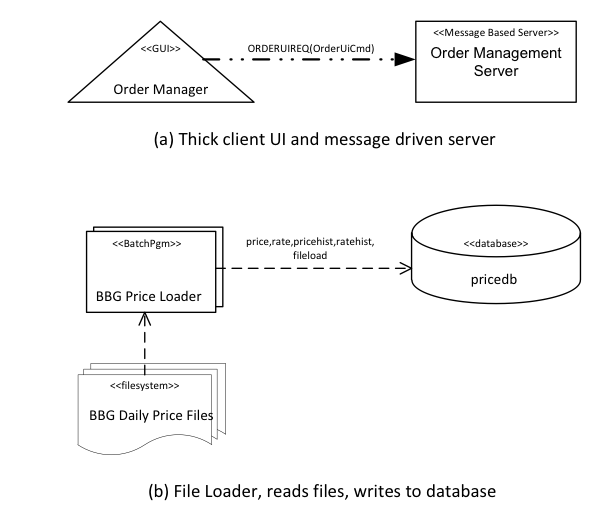
\includegraphics[width=10cm]{Figures/adls-figure1}
\caption{Examples of the ADL Notation Illustrating Preferred Configurations}
\label{figure:adlnotation1}
\end{figure}  

  The notation used to express the examples is explained more fully in the next section, but briefly triangular shapes represent user interfaces, rectangles represent server resident elements (servers, batch programs), files and databases are represented by the fairly conventional "record stack" and "drum" shapes, while connectors are represented by arrows using a variety of line types (the line type in example (a) being messaging, the line type in example (b) being stored data access).

\subsection{The Architecture Description Language}

  Once the universe of required element and connector types was understood, we needed a notation that would allow instances of the style (i.e. the subsystems) to be clearly represented.  As explained earlier, we decided to define a custom notation because the initial discussions with the teams had made it clear that getting people to use a specific tool or invest much effort in learning the notation was going to be very difficult. This was a key reason for creating a very simple notation and "just drawing pictures" rather than trying to apply a general-purpose notation or create machine readable models.

  Given people's general enthusiasm for diagrams over text, we chose to create a graphical notation rather than a more formal textual one. We could have created an equivalent textual notation to provide an alternative concrete syntax, but we didn't need one for this project and as we were not trying to create a reusable ADL we had no reason (or the time) to create alternative notations.

  When defining the graphical detail of the notation, the advice in \cite{moody2009-notations} was particularly useful, in particular the exhortation to avoid construct overload, deficit, redundancy or excess, the suggestion to systematically consider the visual variables of each shape (shape, size, colour, orientation, brightness and texture) and the need for deliberate selection of shapes so that their appearance suggested their meaning, to help achieve semantic transparency.

  We created the graphical notation by selecting a base shape for each major type of element (server, user interface, data store, external entity) and designing a variation of the shape for each subtype of the element.  The diagrams were likely to be printed in black and white, so brightness and colour were used in a very limited way (just being used as an informal diagrammatic annotation, rather than having a predefined meaning).  Each element had to have a name, shown on its symbol and optionally a stereotype (discussed below).  Examples of the notation for some of the more important element types are shown in Figure \ref{figure:adlelementtypes}. 
  
\begin{figure}
\centering
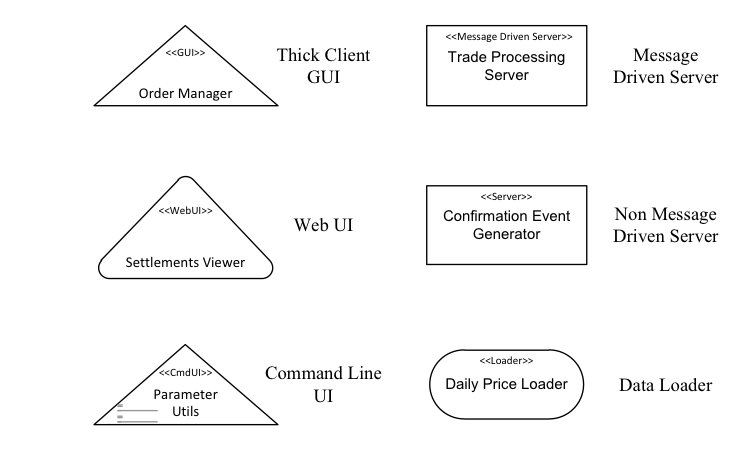
\includegraphics[width=10cm]{Figures/adls-figure2}
\caption{ADL Element Types}
\label{figure:adlelementtypes}
\end{figure}  


  A triangle was used as the base shape for user interfaces and a rectangle for server resident components.  The triangle was chosen as it hinted at the head and shoulders shape of a user and the triangles were then modified slightly for each type of user interface (the thick client having sharp corners, the web user interface having rounded corners as it blurs the distinction between "client" and "server" and the command line utility having a graphical representation of a command line interface added to it).  Similarly, a rectangle is the base shape for server elements (based on long accepted conventions) with a stereotype being used to indicate the type of server and a "lozenge" variant being used to indicate a data loader (hinting at pieces of data being transmitted through it).

  An arrow of some form was used to represent all of the connector types, with the arrowhead usually indicating the direction of data flow.  All connectors were defined to be one way connections, with the exception of data access connectors, which could indicate read and write activity with arrow heads at both ends of the connector if appropriate.  The convention for RPC connectors was defined to be a one-way arrow from the caller to the target.  No attempt was made to represent the various complicated possibilities of dependency and initiation of interaction using the connector symbols.  Each connector had to indicate what was carried over the connection, with message flows being annotated with a message data type, file and database connectors being annotated with table or record names, and RPC and direct invocation connectors being annotated with the name of the service or procedure they were calling.  Examples of the notation for the main connector types are shown in Figure \ref{figure:adlconnectortypes}. 

\begin{figure}
\centering

\includegraphics[width=10cm]{Figures/adls-figure3}
\caption{ADL Connector Types}
\label{figure:adlconnectortypes}
\end{figure}  


  The RPC or direct procedure call is shown using a solid arrow, messaging is shown using a line with embedded dots, suggesting messages flowing over it, while data access is shown using a regular chain line, suggesting records being read or written over the connector.

  A general mechanism used on elements and connectors was the stereotype, adopted from UML, where the type of an architectural element is made clear by annotating it with a type name using the 
convention "{\guillemotleft}type{\guillemotright}" on the symbol concerned.  This allowed the casual reader to understand the types of element on the diagram without having to understand the notation and allowed new element types to be easily introduced.

  The semantics of the elements and connectors were generally based on the semantics of the corresponding element and connector implementations in the system: broadcast messaging in the system worked in a particular way, a relational database has well understood behaviour, a web service call is widely understood and a message driven server was a concept that most people understood with little further explanation.  Undoubtedly there were cases where elements on diagrams had surprising behaviour because they did not behave entirely as expected given their type, but on the whole, the resulting documents were good enough to form a useful architecture description.

  In order to ensure that the process produced more than just pictures, we defined a set of required attributes for each type of element and connector.  Part of this task was defining enumerations of expected standard values for many of the attributes, again to standardise and simplify the process of recording the information (such as standard lists of data domains ["trading", "counterparties", "securities", ...], lists of programming languages in use [C++, Java, C\#, Perl] and so on).

  In order to simplify and standardise the subsystem descriptions, a set of wiki page templates and a comprehensive Microsoft Visio stencil were created, along with clear instructions, quick reference material and - most crucially - a fully worked example of the documentation for one subsystem.  This allowed a number of conventions, such as hyperlinking element names to allow navigation through the documents, to be illustrated and encouraged by example.  A hierarchy of empty wiki pages for the required subsystem descriptions was also created so that authors knew where to put their documents and so they could be unambiguously referenced.

  The result of this process was a relatively informal definition of a simple ADL with a graphical notation and set of well-defined conventions for storing the supporting text needed to explain and fully define the subsystem descriptions.  The ADL is tied very strongly to the particular architectural style of this system (its element and connector types) and we deliberately did not attempt to generalise the language, as this very tight link to the system to be described was one of its major strengths for our situation.  In this way, our ADL is rather like the ADLs defined to support specific implementation frameworks like DAOP-ADL \cite{pinto2003-daopadl} which was developed to describe DAOP applications \cite{pinto2001-daop} and CBabel \cite{rademaker2005-cbabel} which was developed to allow the definition of CR-RIO applications \cite{loques2004-crrio}.

\section{A Case Study of the Approach in Use}

  The system described in the case study is the Asset Management System (AMS) a financial asset management system used by a fund manager to support making and executing investment decisions for a large-scale investment portfolio.  The example is based on a real subsystem from the case study, modified slightly in order to retain anonymity.

  The primary aim of the system is to allow a fund manager (or fund management team) to manage a portfolio of holdings in financial instruments (primarily equities in this case).  The system must allow them to view the content of their portfolios and to use analytical tools and market data (such as prices, volatilities, projected interest and foreign exchange rates and projected bond yields) to make investment decisions.  The system provides the ability for suggested changes to portfolios to be automatically calculated on demand or from a temporal schedule and also allows direct entry of orders to buy or sell securities to allow for investment strategies that are outside the scope of the system.  Once lists of orders to buy or sell securities are generated, the system allows them to be dispatched to another system for execution and it receives the results of the execution of those orders in return, to allow the current holdings to be updated.

\subsection{Architectural Description}

  The functional structure of the AMS is described using our system-specific ADL 
notation in Figure \ref{figure:amsdiagram}. 

\begin{figure}
\centering
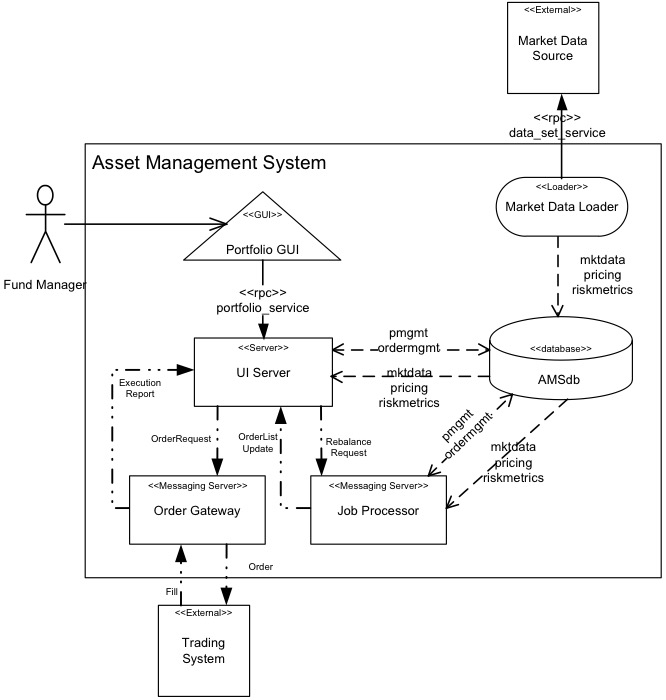
\includegraphics[width=10cm]{Figures/adls-figure4}
\caption{The Asset Management Systems}
\label{figure:amsdiagram}
\end{figure}  

The elements of this architectural structure are described in Table \ref{table:amselements}. 
  
\begin{table}
\caption{Elements of the Asset Management System}
\label{table:amselements}
\footnotesize
\begin{tabular}{| l l p{7cm} |}
\hline
Element Name & Type & Description \\
\hline

Portfolio GUI      & GUI              & The responsibilities of the Graphical User Interface (GUI) are to provide the asset managers using the system with the ability to view and analyse their portfolios, to request (and monitor progress of) long running system operations (such as order generation) and to check, enter, dispatch and monitor orders that go for execution to trading systems.  The GUI provides a human interface and requires an RPC interface to the UI Server to provide it with services and data. \\

UI Server          & Messaging Server & The responsibility of the UI Server is to provide the data access facilities that the UI requires (accessing data from the AMSdb internal database) and to dispatch requests for orders or for long running work (such as analysis processing) to be carried out by other parts of the system.  The UI Server provides an RPC interface to expose its provided services to the GUI and requires an SQL query interface to the system database and a messaging interface to allow it to request and monitor order dispatch and long running work. \\

AMSdb              & Database         & The system database's responsibility is to store the portfolio, analytical, market and (system) operational data that the system requires to operate.  It provides an SQL based DML interface to allow data to be inserted, manipulated or retrieved. \\

Job Processor      & Messaging Server & The responsibilities of the Job Processor are to execute long running processing items ("jobs") such as investment analytics and automated order list generation.  The processor can be configured to run particular jobs on temporal schedules and can also be requested to execute particular jobs on demand.  The processor provides a message based job control and status request interface and requires an SQL query based interface to the database. \\

Market Data Loader & Loader           & The responsibility of the Market Data Loader (MDL) is to retrieve various forms of market data from an internal Market Data Source system and load the data into the database, handling versioning and business date identification as part of the loading process.  The datasets required include securities prices, bond yields, interest rates, FX rates, volatilities, correlations and so on.  The loader requires a data retrieval interface to the MDL system, allowing data sets to be retrieved on demand. \\

Order Gateway      & Messaging Server & The responsibility of the Order Gateway is to accept incoming orders to buy and sell securities (including order parameters such as execution strategies and price limits), to forward these requests to a trading system for execution and then receive the execution reports ("fills") indicating order execution and broadcast these to other interested parts of the system.  The gateway provides a message based order request interface and a broadcast status interface and it requires a message based interface to allow order submission to a trading system.\\
\hline
\end{tabular}
\end{table}

\subsection{Example Scenario - Generate Order List}

  The key functional scenario for this system is to allow a fund manager to generate an order list to "rebalance" a fund based on an analysis that identifies the theoretically optimal holdings for the portfolio and execute that set of buy and sell orders, reflecting the results in the portfolio.  The interactions required to implement this scenario are illustrated in Figure \ref{figure:rebalanceinteractions}. 

\begin{figure}
\centering
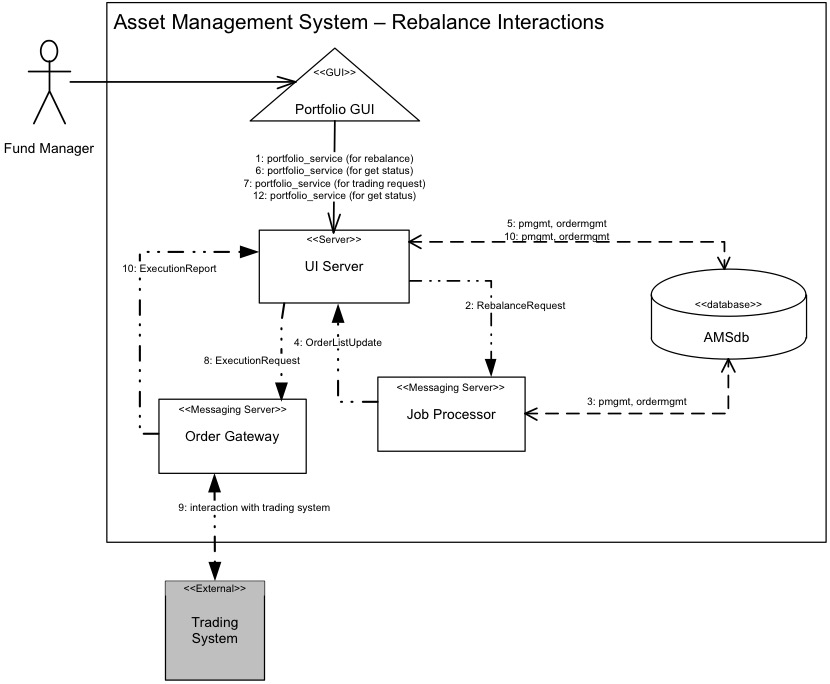
\includegraphics[width=10cm]{Figures/adls-figure5}
\caption{Portfolio Rebalance Scenario Interactions}
\label{figure:rebalanceinteractions}
\end{figure}

The interactions between system elements necessary to implement this scenario are described in Table \ref{table:amsinteractions}. 
  
\begin{table}
\caption{Interactions for the Portfolio Rebalance Scenario}
\label{table:amsinteractions}
\footnotesize
\begin{tabular}{| p{0.5cm} p{2cm} p{2cm} l p{2cm} p{4.9cm} |}
\hline
Step & From & To & Type & Connector & Description \\
\hline

1 & GUI & UI Server & RPC & portfolio service & Fund manager selects a portfolio and instructs the system to create an order list for it.  The GUI invokes an RPC indicating that the indicated portfolio should be rebalanced. \\

2 & UI Server & Job Processor & Msg & Rebalance Request & The UI Server sends a request message to indicate that the portfolio should be "rebalanced".  This is routed to the Job Processor. \\

3 & Job Processor & AMSdb & DB & pmgmt and ordermgmt schemas & The Job Processor receives the message and in response initiates a portfolio analysis job to identify the theoretical optimal holdings in the portfolio and generate buy and sell orders to move the portfolio to that state.  Portfolio state read from "pmgmt" and order lists written to "ordermgmt" \\

4 & Job Processor & UI Server & Msg & OrderList Update & The Job Processor sends a status message indicating that new order lists exist, which is routed to the UI Server \\

5 & UI Server & AMSdb & DB & ordermgmt and pmgmt schemas & The UI Server accesses the database to get the new portfolio state and associated order list state \\

6 & GUI & UI Server & RPC & portfolio service & The GUI calls the UI Server for a status update and gets details of the new order list in return \\

7 & GUI & UI Server & RPC & portfolio service & The GUI makes an RPC call to the UI Server to indicate that the order list should be traded \\

8 & UI Server & Order Gateway & Msg & Execution Request & The UI Server creates a message to request the order list to be traded (including the list of orders) which is routed to the Order Gateway \\

9 & Order Gateway & Trading System & - & - & The Order Gateway sends the orders to an external trading system and receives status updates in return as the orders are executed \\

10 & Order Gateway & UI Server & Msg & Execution Report & As the Order Gateway gets execution updates, it creates execution report messages which are routed to the UI Server \\

11 & UI Server & AMSdb & DB & pmgmt and ordermgmt schemas & The UI Server updates the database with the status of the orders and the effect on the portfolio \\

12 & GUI & UI Server & RPC & portfolio service & The GUI makes RPC calls to the UI Server and gets the updated status of the orders and the changes to the portfolio in its response \\
\hline
\end{tabular}
\end{table}

  A full architectural description for a subsystem would also include a lot of operational and implementation oriented information such as links to operational instructions, links to source code control systems and automated build systems and links to test specifications and results.  We do not attempt to reproduce any of that here as the majority of such information was in the form of links to other internal systems and nearly all of the information is context dependent and so not particularly meaningful outside the organisation operating the system.

\section{Experience Gained}

\subsection{Creating the Architecture Description}

  As mentioned earlier, two experienced architects led the project to create the architecture description, which included identifying the underlying architectural style, defining a clear approach, defining the ADL and leading the work to capture the architectural descriptions.  There were approximately 20 development teams who owned significant subsystems that needed to be included in the scope of the project.

  In order to organise the work, the development teams were ranked in order of the criticality of their subsystems in terms of how central they were to key organisational workflows and this acted as an ordered backlog of work for the architects.

  The general approach taken to the task was simple and involved approaching each team and asking for a single person to be nominated as the owner of their documentation.  A conference call was then held with this person and the group manager to explain the project and the approach.  The team was asked to commit time and effort to completing their documents and to commit to a timeline for completing the agreed deliverables (a team often had a number of subsystems that needed to be documented and for planning purposes the creation of a subsystem description was decomposed into some standard subtasks).  In return, the architects leading the effort offered training, practical assistance (such as drawing diagrams) and to review the descriptions produced.

  The interactions with different teams varied greatly, with some teams producing their documentation largely unaided, needing only some review and minor correction, while others were simply incapable or unwilling to produce what was needed and the architects ended up writing most of the documentation for these teams. 

  The reasons for the problems encountered with development teams varied.  In some cases it was simply a lack of interest, often from the development manager who perhaps didn�t see the value of the deliverables.  However in other cases there seemed to be a genuine difficulty in understanding how to represent their subsystem.  In general this seemed to stem from an inability to abstract away from the implementation, resulting in a confusing mix of concrete and totally abstract concepts, which they then struggled to relate to each other.  None of these subsystems were very difficult to represent and in order to make progress the architects often stepped in and simply created the models.

  Another interesting problem was tooling.  Everyone in the organisation had access to the wiki and knew how to use it, so document authors could fill in the tables and text without any difficulty.  However, not everyone had access to Microsoft Visio and even of those that did, some obviously didn't know how to use it.  Again, the solution to this was simply for the architects overseeing the process to create diagrams for some subsystems.  This was a useful lesson and provided further evidence that avoiding UML and more specialised modelling tools had been a good decision.  In this organisation, requiring the use of UML and modelling tools would have been a significant barrier to getting architectural descriptions created.

  Over time, a significant and useful body of subsystem descriptions emerged and this allowed the architects to create a summary level architecture description that showed how the subsystems related to each other.  Some use of scripting to process the wiki subsystem descriptions and drawing tool macros to generate parts of the summary level diagrams allowed some degree of automation, although it was still a fairly manual process.

   The process of capturing the architecture description took about six months, with the architects working on it approximately 60\% of their time and the development teams working on it as their project schedules allowed.

\subsection{The Results of the Project}

  The outputs of the project were as follows.

\begin{itemize}
\item A fairly consistent architecture description for most of the system that provided an accurate and largely complete view of its subsystems, their components and their dependencies.  Each subsystem was described using a standardised approach, which captured the same information for each one and presented it in a consistent manner through the use of the templates provided.  This made the information provided easy to navigate and check for completeness.

\item An informal definition of the architectural style used across most of the system and the typical patterns used when implementing it.

\item A degree of visibility and understanding of the structure, scale and interconnectedness of the system which hadn't been achieved before.  The consistent presentation of system design information in a single location allowed the overall system structure to be more easily understood compared to the previous inconsistent descriptions on scattered wikis and web sites.  This appeared to allow a number of senior technical managers to achieve new insights into the system.

\item An insight into the degree of implementation uniformity between the different subsystems of the application.  While many subsystems were implemented in a very similar way, like any large system (particularly one which has had other applications integrated into it), parts of this application were implemented in ways that didn't follow the normal set of conventions.  While there was already a general awareness that these less standard subsystems existed, the models made it easier for senior technical staff to gain visibility of this and decide whether they wished to direct any changes to the application as a result.

\end{itemize}

  As mentioned earlier, the project did not have particularly clear goals for the architecture description once developed.  A number of people did find it insightful and there seemed to be a general consensus that it was a useful description to have.  However organisational changes then meant that the architects involved moved on to other work, so the project effectively came to an end.  Since then however another group within the firm has adopted the architectural description and continued its use and maintenance (primarily to support production operation of the system, a use which was not foreseen at the outset of the project).

\subsection{Evaluating the Usefulness of the ADL}

  Early practical experience led to some rapid refinement of the notation to remove ambiguities that had not been apparent to its creators, and to introduce some missing concepts.  However, after three or four teams had used the approach over a period of about 6 weeks, the ADL itself remained stable for the rest of the project.

  As the project neared completion we started to validate what was being produced with some of the important stakeholders, particularly the senior technical managers in the organisation.  To do this we met with them and demonstrated what was being produced and what the completed architectural description would contain, discussing possible uses of it (such as impact analysis, pre-implementation reviews, incident post-mortems and regulatory enquiries).  We were pleased to find that this stakeholder group reacted positively to what they were shown, with responses ranging from fairly neutral (where the possible usefulness was acknowledged but no specific use of it particularly interested them) to very positive (where they wanted to start using it immediately).  Given this informal but consistently positive sentiment, we felt that our notation and approach had been validated (an outcome which was anything but certain at the start of the project, when the use of a specific notation and a highly prescriptive form for the documentation had been viewed as very risky). 

  A factor that was constant throughout the project was that teams who had the ability to identify clear abstractions for their subsystems also appeared to find the ADL helpful and straightforward to use, as the ADL gave them a clearly defined way to represent their models and they didn't have any difficulty in representing their models using it.  These teams tended to create their models with little or no assistance once they'd asked a few clarifying questions about the purpose of the models and the semantics of the notation.

  In contrast, teams who struggled to identify good abstractions never really grasped how to use the ADL and needed constant assistance, to the point of needing to have parts of their architectural descriptions completely rewritten for them.   What was interesting about this stark contrast in modelling ability was that we could find no obvious factor to explain it in terms of educational background, age, team size, technology preferences, type of subsystem, geographical location or any other relevant factor.  We did observe that even in teams that produced good models, the ability and enthusiasm to do this varied and even for large subsystems we found that it tended to be one or two people in a team who did all of the modelling on behalf of the rest of the team.  We don't know whether there were many other people in those teams who would have done an equally good job, but based on hallway conversations, we suspect not.  Our conclusion was that relatively few people in the general population of software engineers we worked with find modelling straightforward, but we were not sure why this was the case.

  We interpreted this experience as validation of the approach that had been used.  People who could create models and knew what they wanted to represent were able to use the ADL effectively with minimal training, so it was obviously usable by mainstream practitioners.  On the other hand, the approach did not help those people who found it difficult to create a model.  It had been hoped that the straightforward and prescriptive nature of the approach would guide people to create useful models, even if they did not find modelling easy, and it was a disappointment that the approach failed to achieve this.

  \section{Lessons Learned From The Project}

  At the start of the project, no one involved in it had much experience in using ADLs in a large-scale industrial context.  Our experience was limited to the use of ADLs in an academic context and some significant experience of using UML for architectural modelling in large industrial projects.  Therefore, we had relatively few preconceptions as to how successful the project would be and on the whole we judged it to be a success.

  The main lessons that were learned during the course of the project were:
  
\begin{itemize}

\item A specialised ADL can have benefits over a general modelling language like UML and even a simple ADL can be used to create useful results.

\item The more specialised an ADL is, and so the closer it matches the implementation style of the system being modelled, the easier people seem to find it to use.  While at first glance this sounds like an obvious point, it is contrary to the conventional industrial approach of using a general modelling language like UML or SysML and also contrasts with the domain independent nature of most academically developed ADLs.

\item Carefully designing the detail of the graphical notation pays off.  Using shapes that hint at their meaning and using a range of graphical dimensions to differentiate shapes helps people to remember them, even if they don't guess the link between the shape and the concept themselves.  Again, this is not reflected in mainstream notations like UML or most existing ADLs, where little effort is made to identify meaningful symbols for concepts.

\item Consistency in the notation is very important and having a base shape for a general concept with refinements to it for different sub-concepts appears to help people considerably when interpreting the diagrams.

\item Providing high quality support materials including an example-based description of the approach and notation, a number of realistic completed examples and a set of templates for new documents is very important.  We found repeatedly that people are much better at "filling in the gaps" rather than following a set of instructions and creating something from scratch.

\item Utilising familiar tools helps with the acceptance of the approach.  In this particular organisation, there were no complaints or difficulties with the use of a wiki for the text and tables information, whereas a very widely used commercial drawing tool (Visio) caused problems, even with a carefully tailored template, because it was not widely used in the organisation already.

\end{itemize}

  These lessons aren't all that surprising but the importance of what seemed to be quite minor things (such as worked examples and quick reference cards) is important and is useful to bear in mind for the future.  The importance of matching the ADL to the specific domain being modelled is also a lesson that is not reflected in most modelling languages today, which tend towards the general rather than the specific.  

  \section{Validation} 
  \label{section:adlvalidation} 

  The goal of this work was to establish whether an ADL could be used to capture the architectural structure of a complex system so that the architectural description could be used to reason about the architectural properties of the system such as performance, resilience, modifiability or energy efficiency.

  Looking back to the specific goals we set at the start of the work, we considered whether the architectural description we had created was a useful catalogue of the current state, could allow the architecture to be understood to allow estimation of qualities such as its energy properties, to provide a tool for impact analysis and to provide a reference to communicate the architecture of the system (see Section \ref{sec:overview}).
  
\begin{itemize}

\item Create a Catalogue of the Current State - the project created the first comprehensive description of the system and so provided a very useful descriptive catalogue of the current state of the architecture.  The weakness of the architectural description as a catalogue was that it was only as comprehensive as the authors of each piece decided to make it.  However, it was possible to cross check it against a number of systems that were known to contain complete lists of the elements in the production system (as they were used for automated tasks relating to deployment).  Sampling about 30 percent of the architectural description and cross checking this against the lists of deployment elements revealed a high degree of completeness, so confidence in its use as a catalogue was high.

\item Allow Architectural Characteristics to be Estimated - as described earlier, the architectural description comprised a diagram and a set of tables and text for each major component within the system.  While this was an effective representation for human use and was useful for impact analysis (see below) it was not all that effective for any sort of architectural quality assessment, such as energy properties of a component.  This was because of the fundamental tradeoff between the flexibility, accessibility and usability of the notation and its formality.  While we were successful at enforcing conventions for the graphical models and for the representation of descriptive text and tables, it would not have been possible to persuade the development teams to use a formal,  checked notation.  Therefore we concluded that while the architectural description could have many uses, it would not be realistic to use it for any sort of automated architectural analysis.

\item Allow Impact Analysis - the architectural description quickly proved its worth for impact analysis and helped considerably with the process of understanding the impact of proposed changes.  This was primarily due to the fact that it allowed the interconnectedness of system elements to be quickly assessed, information that hadn't been easy to find before.  An example of this was a small project to migrate the interface to an important internal service from a legacy RPC technology to the currently strategic message based interface.  The service interfaces were designed so that they could be used in parallel and the plan was to offer both and then slowly migrate users of the service to the new version.  The problem with this was the time it was going to take to find all of the users of the service and so the length of time that the parallel interfaces would be needed.  The model was in a late state of development when this project started to think about migration and they were able to use it to discover nearly all of the clients of their service.  So rather than relying on a service provider keeping track of the users of the service, the model provided a structure to allow the users of the service to declare their interest in the services they used, which was a much more effective approach.

\item Communicate - the architectural description was quickly recognised to be a comprehensive knowledge base of the system's design information and so helped inter-team communication (when people in one team could use it to understand another team's subsystem).  An example of the model being used for this sort of collaboration was when a new application, which had been acquired as part of the acquisition of another firm, was being integrated into the existing application as a new subsystem.  The existing models helped the new team see how existing subsystems were integrated with each other and the model that the new team created of their subsystem helped the existing teams to understand what was being added to the system and how it might be used.  The architectural description also acted as a single place where further information could be gathered.  As mentioned earlier, the architects involved in creating the architectural description moved onto other work soon after its initial creation, however it does appear to have continued to be used, to grow and to evolve, suggesting that it did fulfil this role.  Eventually it was adopted by the Production Services team in the firm, due to the value that they got from having up to date descriptions of the structure and dependencies of each application, for support tasks.

\end{itemize}

  We judged the project to have met the most of the goals we set for ourselves and in particular we met the goal to create a useful shared architectural description and this was confirmed as it became a useful resource within the organisation, within a couple of months, acting as a centralised and standardised source of design information for the system.

  Given the relative success of this project, it is natural to ask how generally applicable its results are and how repeatable it is likely to be.  Given what we learned during the project, particularly the fact that the specialised nature of the notation was a key factor in its success, we feel that these lessons may well have general applicability, but only in the broad sense.  People like to be guided, they like familiar tools and techniques and they are unwilling to learn and use formal languages for design and architectural description.  However the specific tools or techniques that work will be specific to each environment and people in different environments will have different levels of enthusiasm for learning new approaches.  However, when trying to get a significant amount of work done by people who are agnostic to the approach, familiarity and accessibility appear to help greatly with acceptance.

  Based on our experience, the specific suggestions that we would make for future modelling languages are as follows:

\begin{itemize}
\item Create a language that is specific to a domain (e.g. real-time control systems or enterprise information systems) and ensure that it contains the type of modelling elements needed in that domain.  Modelling languages also need to be easily extensible by their users, rather than modelling language experts, to allow missing element types to be added.  Of course specialising a language limits its possible user community, but conversely that user community is more likely to find a language that matches their problems useful and so are more likely to use it.

\item Spend time creating a rich visual notation that communicates as much as possible using the shape, line, fill and other visual aspects of the notation.  This makes diagrams much easier for people to understand.

\item Keep modelling languages as simple as possible so that people can start using them quickly without a great deal of training.  We have observed that modelling language constructs with complex or obscure semantics are rarely used correctly, if they are used at all.

\item Consider how people will use the language and what they will need in terms of tools and facilities for structuring and managing large models.  Again simple tools (and ideally extensions to tools that people are already likely to be familiar with) are much more likely to be successful than tools that require a lot of training and experience to use.

\item As well as the language and tools, develop the materials that people will need in order to successfully adopt the language for practical use.  This includes task oriented training material, quick reference guides and plenty of samples which show the value of the language in use and provide people will examples of how to use it well (which they will almost certainly copy).
\end{itemize}

  It is worth noting that our experiences from this work and our resulting suggestions are similar to the conclusions of a major academic survey of practitioner requirements for 
  ADLs \cite{malavolta2013-industryadlneeds}, which suggests that these lessons and requirements reflect the needs of a significant number of industrial software architects.

  Beyond the experience we have gained in applying architectural description techniques to a large scale problem, the particular notation and approach used in this paper may be of use to others, but as explained earlier in the paper, this wasn't a goal of the project. While some of the aspects of the notation invented will be generally familiar (e.g. servers that are driven by messaging) the overall set of element types is specific to one environment and may well not be directly useful elsewhere.  Certainly we did not set out to contribute yet another general purpose ADL to the world and so reuse of the notation was not considered during its development.  We report this project in order to describe a successful application of the concepts of architectural description notations, to record the factors that we believe made the project successful and to capture the lessons learned and conclusions drawn from the experience.

\section{Summary And Conclusions}

  In order to investigate the practicality of using an ADL to describe a complex architecture, we worked with an organisation in the financial services industry  to create an architecture description for a large existing enterprise system.  In order to achieve this within acceptable cultural and time constraints existing ADLs from the research domain proved to be unsuitable and so a simple, very specific architecture description language was defined in order to make the process of capturing the architecture description as simple and prescriptive as possible.

  While it was not clear at the outset whether this approach would be successful, the ADL proved to be a helpful and effective tool for capturing this specific architecture description in an entirely industrial context.  A large architecture description was created, something that the organisation had not achieved before, and this allowed new perspectives on the system to be gained.

  The factor that appeared to make the approach generally successful was focusing on describing the specific structures in the system of interest, rather than trying to create a general-purpose approach, which would be effective for other uses too.  Other factors which contributed to the success of the approach were its simplicity (which traded sophistication for accessibility), a carefully designed, consistent graphical notation, the availability of a large amount of tutorial and reference material to guide document authors, and the use of very familiar tools, which users of the notation were already familiar with.

  What the case study did not achieve was the ability to describe the architecture in a sufficiently precise manner to allow its qualities to be analysed and so its qualities, such as energy properties, to be estimated.  We found that there was a fundamental trade off between creating an ADL simple and specific enough for mainstream practitioners to use, versus using an ADL from the research domain that, while rigourous, was too general purpose, abstract and complex for mainstream practitioner use.  Our conclusion from this exercise is that existing ADLs are not a practical tool for use in the analysis and estimation of system energy properties.


